\documentclass[11pt]{article}
\usepackage[utf8]{inputenc}
\usepackage[english, ngerman]{babel}
\usepackage{amsmath,amsthm,verbatim,amssymb,amsfonts,amscd}
\usepackage{enumerate}
\usepackage{listings}
\usepackage{courier}
\usepackage[]{graphicx}
\usepackage[]{epstopdf}
\usepackage[margin=1in]{geometry}
\lstset{
  numbers=left,
  language=C,
  basicstyle=\footnotesize\ttfamily,
  breaklines=true,
  morekeywords={function, NIL}
}
\newcommand{\abs}[1]{\left| #1 \right| }
\setlength{\parindent}{0pt} 

\author{
  Felix Schrader, 3053850 \\ 
  Jens Duffert, 2843110 \\
  Eduard Sauter, 3053470
}
\title{Datenstrukturen und Algorithmen: Haus\"ubung 6}
\begin{document}
\maketitle
  \subsection*{Aufgabe 1}
  \begin{enumerate}[a)]
    \item $ $
      \begin{figure}[h!]
      \centering
      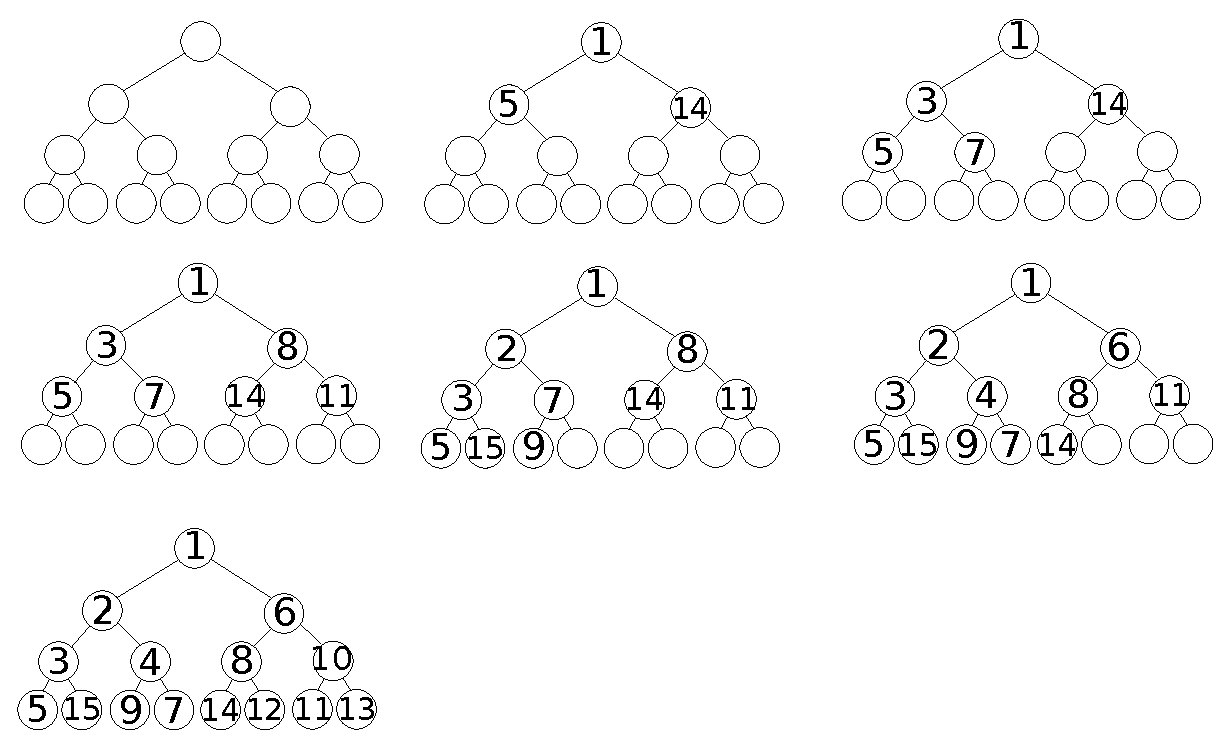
\includegraphics[width=\textwidth]{a1a_trees}
      \caption{Zwischenschritte der Konstruktion des Heaps aus dem gegebenen Schlüssel}
      \end{figure}
    \item $ $
      \begin{figure}[h!]
      \centering
      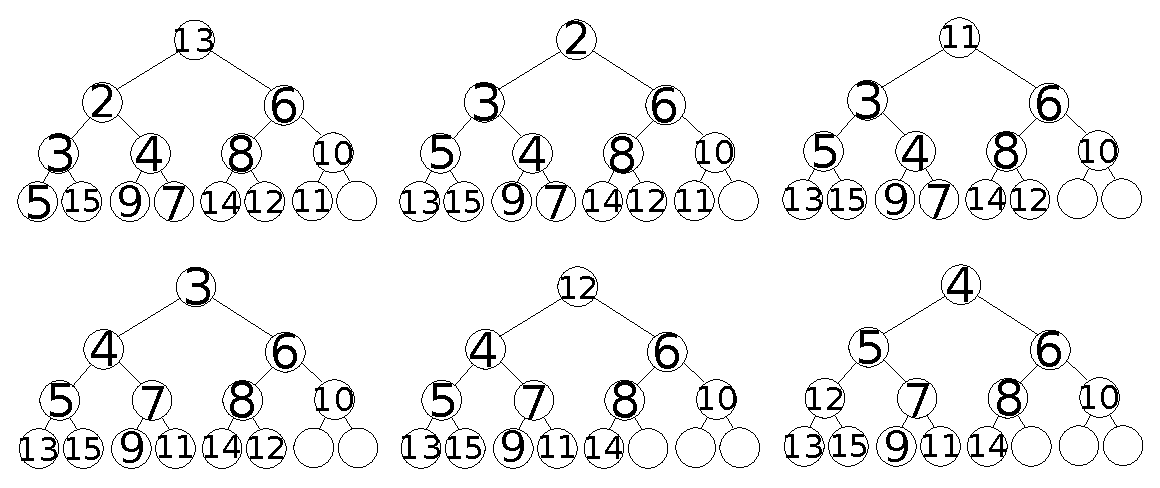
\includegraphics[width=\textwidth]{a1b_trees}
      \caption{Heap nach Entfernen der Wurzel und Sortieren}
      \end{figure}
    \pagebreak
    \item $ $
      \begin{figure}[h!]
      \centering
      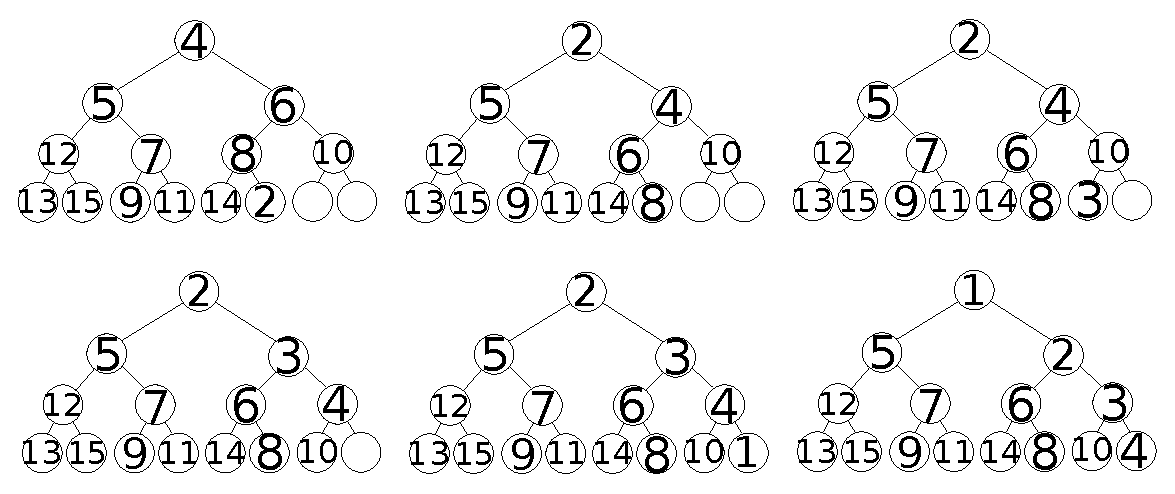
\includegraphics[width=\textwidth]{a1c_trees}
      \caption{Heap nach Hinzufügen von 2, 3, 1 und Sortieren}
      \end{figure}
  \end{enumerate}

\end{document}
